% Manuscript: Classical infrared correlation rules as diagnostic tests
% Build: latexmk -pdf main.tex   (or upload the paper/ folder to Overleaf)
% Journal templates (Applied Spectroscopy, SAGE) are applied at submission;
% this file uses the plain article class so that the text can be moved.
\documentclass[11pt,a4paper]{article}

\usepackage[utf8]{inputenc}
\usepackage[T1]{fontenc}
\usepackage{lmodern}
\usepackage[margin=2.5cm]{geometry}
\usepackage{graphicx}
\usepackage{booktabs}
\usepackage{longtable}
\usepackage{array}
\usepackage{amsmath}
\usepackage{textcomp}
\usepackage{microtype}
\usepackage[numbers,sort&compress]{natbib}
\usepackage{lineno}
\usepackage{setspace}
\usepackage[hidelinks]{hyperref}
\usepackage{xcolor}

\graphicspath{{figures/}}
\linenumbers
\onehalfspacing

% units and symbols used throughout
\newcommand{\wn}{cm$^{-1}$}
\newcommand{\LRp}{LR$^{+}$}
\newcommand{\LRn}{LR$^{-}$}
% editorial notes to ourselves; remove before submission
\newcommand{\todo}[1]{\textcolor{red!70!black}{[#1]}}

\title{Classical infrared correlation rules as diagnostic tests:\\
likelihood ratios from 6,663 experimental spectra}

\author{Kementsu Ibarguen Calvo\\
\small Mol Insight S.L., Bilbao, Spain\\
\small \texttt{kementsuibarguen@gmail.com}}

\date{}

\begin{document}
\maketitle

% Abstract: written last in practice; this is the working draft built from
% the four ideas in the author's Spanish outline (origin, what was done,
% the two regimes, what the tables leave unsaid). Target 250 words.
\begin{abstract}
Infrared correlation tables give, for each functional group, a wavenumber window and an adjective. They do not say how often a band is found in that window when the group is absent, and that is the number that decides whether the observation is evidence. We treated every published rule as a diagnostic test. A set of 101 rules for 60 functional groups, transcribed from one widely used interpretation course and frozen before any confirmatory analysis, was scored on 1,539 ATR spectra of synthesised compounds from the Chemotion repository and replicated on 5,124 transmission spectra from the NIST Chemistry WebBook, with the deposited structure as ground truth and sensitivity, specificity and likelihood ratios as the metrics. The main result is a division of the spectrum into two regimes. Above 1500~\wn{} most rules carry real evidence (median positive likelihood ratio 2.8 and 3.0 in the two collections, up to 43 for the saturated ester carbonyl); in the fingerprint region, at or below 1350~\wn{}, band position alone is close to uninformative (median 1.1 and 1.2), because almost every spectrum has a band in almost every window. The rankings agree across the two collections (Spearman 0.79; 87\% of rules within a factor of two). The audit also measures what the tables leave unsaid: intensity qualifiers cost more sensitivity than they buy specificity (the nitrile band reaches the stated intensity in one nitrile in ten), the benzene substitution patterns do not reach a likelihood ratio of 5 in either collection, and several rules are far more useful for ruling a group out than for ruling it in. We provide the quantified table, the frozen rule set and the scripts so that the audit can be extended to further rules and collections.
\end{abstract}

\noindent\textbf{Keywords:} infrared spectroscopy; correlation tables; group frequencies; functional group identification; likelihood ratio; diagnostic accuracy; open spectral data

\section{Introduction}
\label{sec:intro}

A correlation table is the first instrument of infrared interpretation. It lists, for each functional group, the wavenumber range in which a band is expected, together with a word or two about its intensity and shape, and it is where every chemist starts when a spectrum has to be read without a reference compound. The tables have a long lineage, from the compilations of Bellamy and of Colthup, Daly and Wiberley~\cite{bellamy1975infrared,colthup1990introduction} to the practitioner's summaries in current use, among which Smith's column in \emph{Spectroscopy}~\cite{smith2025bigreview4,smith2026bigreview8} is one of the most widely read. Their entries were derived from curated spectra of known compounds, refined by decades of experience, and they are for the most part right.

What the tables do not carry is a measure of how much each entry is worth. A rule of the form ``ester, C=O stretch, 1735 to 1755~\wn{}, strong'' says where the band is when the group is present; it does not say how often a band is found there when the group is absent, and that second number decides whether the observation is evidence. The tables could not give it, because they were built from spectra that contain the group, and a collection of positives has no denominator. The reader supplies the missing judgement from experience, and the experience is real, but it has not been written down, and it does not transfer to a student on the first day or to a program that applies the table one row at a time. We met the problem in that form, when encoding the tables as rules for automated interpretation: several entries, applied literally, disagreed with each other and with experimental spectra of compounds that unquestionably contained the group.

The gap has been felt before. The rule-based interpreters of the 1980s and 1990s, PAIRS and EXPIRS among them~\cite{woodruff1980pairs,woodruff1981rules,andreev1996expirs}, encoded correlation tables as rules with a confidence attached to each one; those confidences were set by the spectroscopist who wrote the rule, because collections large enough to measure them did not exist. More recent work trains neural networks on spectral collections to predict functional groups directly~\cite{fine2020spectral,punjabi2025chemotion} and reports the accuracy of the model, not the value of any rule a chemist could read. To our knowledge, no published correlation table has been scored rule by rule on experimental spectra of known structure, which is what this paper does.

Two things make it possible to measure the rules now. Open collections of experimental spectra with the depositor's structure attached have become available: the Chemotion repository has released several thousand ATR spectra from synthesis laboratories under an open licence~\cite{punjabi2025chemotion}, and the NIST Chemistry WebBook holds several thousand condensed-phase transmission spectra with structures~\cite{nist_webbook}. And the language for the question already exists. A correlation rule is a diagnostic test: it has a positive and a negative outcome, a target condition and, given a collection with known structures, a sensitivity, a specificity and a pair of likelihood ratios that say how much a positive or a negative result should shift the odds of the group~\cite{deeks2004likelihood}. Likelihood ratios are the natural currency because they are what a reader combines with what is already known about the sample, and because they can be compared across rules and across collections.

This paper reports such a measurement. A set of 101 rules for 60 functional groups was transcribed from one source, frozen before any confirmatory analysis, and scored on 1,539 ATR spectra from Chemotion and 5,124 transmission spectra from NIST, with the deposited structure as ground truth. We report, for every rule, its sensitivity, specificity and likelihood ratios in both collections, the effect of the intensity and shape qualifiers the source attaches, and a failure analysis that says what fills each window when the rule does not discriminate. The result is a quantified version of a table that has so far carried only positions and adjectives.

Three things the study does not do should be said at the outset. It does not propose new rules or adjust the published ones: every window and qualifier is scored as printed, and where it disagrees with the data the disagreement is reported. It does not model interpretation as an experienced reader performs it, weighing bands against one another; each rule is tested on its own, which is the form in which tables are taught and programmed. And it does not claim that any particular source is wrong. The source we used is the one we consider best documented; the method applies to any other unchanged, and the scripts and the frozen rule set are released so that it can be.

\section{Methods}
\label{sec:methods}
% Every operational choice needed to reproduce the numbers, in the order the
% data flows. The development split is mentioned once; no development number
% is reported.

\subsection{Rule set}
\label{sec:rules}

The rules were taken from a single, widely read source: the ``IR Spectral Interpretation Workshop'' column by Brian C. Smith in \emph{Spectroscopy}, in its five ``Big Review'' summaries (hydrocarbons, the C-O bond, carbonyl compounds in two parts, organic nitrogen compounds)~\cite{smith2025bigreview4,smith2025bigreview5,smith2025bigreview6,smith2025bigreview7,smith2026bigreview8} and seven topical columns on benzene rings, alkenes, alkynes, aldehydes, nitriles, nitro groups and amine salts~\cite{smith2016benzene,smith2016alkenes,smith2017alkynes,smith2017aldehydes,smith2019nitriles,smith2020nitro,smith2019aminesalts}. We chose one source rather than a compilation because the study needs each rule to be exactly what one author wrote, with its window, its intensity word and its conditions, and because these columns are the reference many practising chemists use today. The tables were transcribed into a machine-readable form: one row per rule, with the group it refers to, the lower and upper wavenumber of the window, the intensity (``strong'', ``medium'' or unstated) and shape (``sharp'', ``broad'' or unstated) qualifiers as printed, and, for the benzene substitution patterns, the second window the rule requires or forbids. Where the source gives a centre and a tolerance the window is the centre plus and minus the tolerance; the one rule given as an approximate centre with no tolerance (secondary aromatic amine N-H, ``about 3400'') was assigned the 40~\wn{} width of its neighbours in the same table, and this is the only value not printed in the source.

The table holds 106 rules. Four refer to cis and trans alkenes and cannot be scored because most deposited structures carry no stereochemistry, and one (the overtone and combination bands of amine salts) covers three salt types and has no single structural target; these five are kept in the table as not evaluable. Of the 101 evaluable rules, 86 refer to a specific group in the main stratum, 7 to protonated amines and are scored in the salt stratum only, and 8 are umbrella rules (``any carbonyl, 1600 to 1900'') that the source uses as a first pass; these are scored against union groups and reported in their own tier, not compared with group-specific rules. Thirty-one rules state an intensity and 13 a shape.

The table was frozen, together with every choice described below, before the confirmatory data were examined, and the frozen version is tagged in the repository (\texttt{rules-frozen-v1}). No window, qualifier or threshold was changed afterwards; where a rule disagrees with the data, the disagreement is reported.

\subsection{Ground truth}
\label{sec:truth}

A spectrum is positive for a group when the depositor's structure contains a substructure that matches a SMARTS pattern for that group. Seventeen patterns were taken from Punjabi et al.~\cite{punjabi2025chemotion}, who adapted them from Fine et al.~\cite{fine2020spectral}; 43 were written for this work so that every evaluable rule has a target that means what the source means. The definitions follow the source's own words as literally as possible: a primary alcohol is a hydroxyl on a CH$_2$; ``saturated'' means that the atom attached to the group is sp$^3$ and ``aromatic'' that it is aromatic, so the two classes are exclusive and neither includes $\alpha,\beta$-unsaturated carbonyls, which count only for the parent group; amines and amides exclude N-N, N-O and acyl nitrogen. The 60 patterns are listed in the Supplementary Information and in the repository, with the number of matches in each collection.

Structures were standardised with RDKit~\cite{rdkit} (largest fragment for the main stratum, charges as deposited) and identified by InChIKey. The ground truth is therefore the structure the depositor recorded; we did not verify structures against the spectra, since that would presuppose the rules under test. Deposition errors exist; their expected effect is to add noise and to lower measured performance, not to favour any rule.

\subsection{Spectral collections}
\label{sec:data}

\paragraph{Chemotion.} The primary collection is the open IR dataset released with the Chemotion repository~\cite{punjabi2025chemotion} (RADAR4Chem, CC BY-SA 4.0), 4,183 JCAMP-DX files from synthesis laboratories, deposited between 2016 and 2024, each linked to the depositor's structure. Nearly all were recorded on Bruker Alpha ATR instruments with a diamond crystal at 4~\wn{} resolution, from 374 to 3997~\wn{}; the collection is an ATR collection and its intensities carry the ATR wavelength dependence. Chemotion exports each measurement twice (raw and peak-picked), so one file was kept per analysis; files without data points, with fewer than 500 points, not covering 650 to 3800~\wn{}, with constant intensity or with an unparsable structure were removed. This left 2,113 spectra of 1,921 distinct structures. Spectra of metal complexes (150) were excluded; spectra of salts and other multi-fragment entries without metals (40) form a salt stratum used only for the amine salt rules, and the remaining 1,923 spectra form the main stratum.

Twenty percent of the distinct structures (seed 20260914) were set aside as a development set on which the pipeline was built and checked; duplicates of one structure never straddle the two sets. All decisions in this section were taken on the development set. The confirmatory set, 1,692 spectra of which 1,539 are in the main stratum, was analysed once, after the freeze, and is the only Chemotion set reported.

\paragraph{NIST.} The replication collection is the infrared section of the NIST Chemistry WebBook (Standard Reference Database 69)~\cite{nist_webbook}, from which every condensed-phase spectrum with data points was retrieved with a script that is provided with the repository (the spectra themselves are subject to NIST's terms of use and are not redistributed). These are transmission spectra, mostly from the Coblentz Society and NIST collections recorded before 1990 on grating or prism instruments, of KBr discs (1,742 of the primary spectra), mulls (1,360), solutions (1,254) and neat liquids or films (1,126). Records were kept if the abscissa was in wavenumber or micrometres (the latter converted), the ordinate in transmittance or absorbance, the state condensed, the range covering 700 to 3800~\wn{} after conversion, and a structure available from the WebBook; 5,894 spectra passed. Where a species had several spectra one was kept, preferring wavenumber over micrometre abscissae (which are digitised and resampled) and, in order, KBr, liquid, solution and mull preparations. The main stratum holds 5,124 spectra of 5,122 structures; 66\% contain an aromatic ring, against 93\% in Chemotion. Because many prism-era spectra begin at 650 to 700~\wn{}, each rule was scored only on the spectra whose measured range covers every window it uses; this rule was applied to both collections and changes nothing in Chemotion.

\subsection{Processing and band detection}
\label{sec:bands}

Spectra were converted to absorbance ($A = -\log_{10} T$, with $T$ floored at $10^{-4}$), interpolated onto a 2~\wn{} grid from 400 to 4000~\wn{}, and baseline-corrected with asymmetric least squares~\cite{eilers2005baseline} (smoothness $10^6$, asymmetry 0.001, ten iterations), which follows the underside of the spectrum without cutting into bands. Each spectrum was then scaled so that its strongest point between 650 and 3800~\wn{} equals 1; every intensity in this work is relative to that point. Bands are the local maxima of the corrected spectrum with a prominence, the height above the higher of the two flanking minima, of at least 0.01; each is described by its apex position, its height relative to the strongest band and its full width at half prominence. Intensity classes follow the three levels of the source: strong, at least 0.6 of the strongest band; medium, at least 0.2; weak, below. Shape classes use the width: sharp below 30~\wn{}, broad from 30 to 100, very broad above.

The prominence threshold at which a candidate counts as a band is the one parameter with a visible effect on the results, and it was fixed on the development set: 0.02 of the strongest band is the primary value, because real diagnostic bands in this collection can be that weak (the C$\equiv$N stretch of Section~\ref{sec:nitrile} is the example), and 0.01 is at the noise floor of some spectra. Every result was also computed at 0.01, 0.05 and 0.10, and the sweep is given in the Supplementary Information.

\subsection{Scoring a rule}
\label{sec:scoring}

A rule is satisfied by a spectrum when a band with prominence at or above the threshold has its apex inside the window and, in the full definition, its intensity class and shape class match the qualifiers the source states (a ``medium'' qualifier accepts strong or medium; a ``broad'' qualifier accepts broad or very broad). Three nested definitions were computed for every rule, position only, position with intensity, and position with intensity and shape; the full definition is primary because it is what the source says, and the position-only result is reported alongside it. For the benzene substitution rules, a required second window must also contain a band and a forbidden window must contain none, at the same threshold. Each rule was scored on the spectra of its stratum whose measured range covers all its windows.

\subsection{Statistics}
\label{sec:metrics}

For each rule and definition a 2$\times$2 table was formed from the rule outcome and the ground truth, and sensitivity, specificity, predictive values and the positive and negative likelihood ratios~\cite{deeks2004likelihood} were computed, with 95\% confidence intervals on the logarithmic scale~\cite{simel1991likelihood} and a continuity correction of 0.5 when a cell was empty. Because spectra of related compounds are not independent (the 1,923 Chemotion spectra fall into 545 Murcko scaffold~\cite{bemis1996murcko} families, the largest holding 193 spectra), a second interval for \LRp{} was obtained by a cluster bootstrap that resamples scaffold families rather than spectra (500 resamples, fixed seed); it is the interval shown in the figures. Rules with fewer than ten positive spectra in a collection are reported but marked underpowered and not interpreted. For each rule with at least five false positives, the groups over-represented among the false positives relative to the true negatives were listed by odds ratio, as the basis of the failure analysis. No correction for multiple comparisons was applied and none is needed: the study estimates a likelihood ratio for each rule and does not test whether any rule is ``significant''. Four hypotheses about the pattern of results were written down before the confirmatory run and are given, with their outcome, in the Supplementary Information.

\subsection{Software and availability}
\label{sec:software}

The pipeline is written in Python with RDKit~\cite{rdkit} for substructure matching and scaffolds, SciPy~\cite{virtanen2020scipy} for baseline correction and peak detection, and the jcamp package for file parsing. The frozen rule table, the SMARTS definitions, all scripts, the list of NIST identifiers used and the per-rule result tables at every threshold and definition are available at \url{https://github.com/Kementsu/ir-correlation-rules-paper}, tagged \texttt{rules-frozen-v1}. The Chemotion spectra are available from RADAR4Chem; the NIST spectra can be re-downloaded with the script provided. A large language model was used to draft text and analysis code under the author's direction, as stated in the declaration at the end of the article.

\section{Results}
\label{sec:results}
% One subsection per figure, in the order of the argument:
%  3.1 the two regimes (Fig. 1, Table 1)   3.2 the intensity clause (Fig. 2)
%  3.3 the nitrile (Fig. 3)                3.4 benzene patterns (Fig. 4)
%  3.5 rule-out value (LR-)                3.6 replication (Fig. 5)

After quality control and the one-spectrum-per-structure rule, the confirmatory Chemotion set contained 1,539 spectra in the main stratum and the NIST set 5,124. Of the 101 evaluable rules, 73 had at least ten positive spectra in Chemotion and 85 in NIST; the remaining rules are reported in Table~\ref{tab:rules} but not interpreted. Unless stated otherwise, all figures below refer to the primary band-detection threshold and to the full rule definition, that is, position together with any intensity or shape qualifier the source gives.

\subsection{Two regimes of the spectrum}
\label{sec:regimes}

Figure~\ref{fig:regions} plots the positive likelihood ratio of every powered rule against the centre of its published window, and Table~\ref{tab:summary} counts the rules in each \LRp{} band by region. The two collections give the same picture. Rules whose window lies at or above 1500~\wn{} have a median \LRp{} of 2.8 in Chemotion and 3.0 in NIST; rules whose window lies at or below 1350~\wn{} have a median of 1.06 and 1.21. In the upper region 7 of 31 Chemotion rules and 9 of 37 NIST rules reach \LRp{} 5, the level that the diagnostic literature uses, by convention, to mark a test whose positive result carries substantial weight on its own~\cite{deeks2004likelihood}; in the fingerprint region none of the 38 or 43 rules does, and 26 of 38 in Chemotion (21 of 43 in NIST) fall below 1.2, where the band is found almost as often without the group as with it. The handful of rules whose window straddles the boundary (4 and 5) behave like the fingerprint.

The rules that carry most evidence are the ones a spectroscopist would name first. In Chemotion the seven rules above \LRp{} 5 are the saturated ester carbonyl (43), the aromatic nitrile (189, but see Section~\ref{sec:nitrile}), the two asymmetric NH$_2$ stretches of primary amines (8.7 alkyl, 6.8 aryl), the aromatic ester and saturated ketone carbonyls (6.1 and 5.9) and the asymmetric nitro stretch (5.3). NIST, whose composition gives power to groups that Chemotion lacks, adds the three organic carbonate carbonyls (5.7 to 9.6), the saturated aldehyde carbonyl (6.3) and the terminal alkyne C$\equiv$C (12), and keeps the saturated ester carbonyl (12) and the nitriles at the top. Below 5 but above 2 sit most of the remaining carbonyl, N-H, O-H and C$\equiv$C rules, together with the C-H stretches of methyl and methylene groups.

The fingerprint tells a different story. Its rules are not failing to find the band: the median sensitivity of the 38 Chemotion fingerprint rules is 0.90, higher than the 0.47 of the rules above 1500~\wn{}. What they lack is specificity, a median of 0.16 against 0.85, and for 15 of the 38 it is below 0.10. The C-O stretch of secondary alcohols (1075 to 1150~\wn{}) illustrates the pattern: 94\% of secondary alcohols show a band in the window, and so do 95\% of the compounds that are not secondary alcohols, for an \LRp{} of 0.98. The same holds for the C-O of phenols, ethers and acids, the C-N of amines and amides, and the out-of-plane C-H bends of alkenes and benzene rings. The region is simply crowded: at the primary threshold a typical Chemotion spectrum carries 16 detected bands between 700 and 1350~\wn{} (interquartile range 13 to 18), enough to occupy 85\% of the 50~\wn{} windows in that range, against 10 bands in the whole region above 1500~\wn{}. A rule that asks only whether a band is present in a fingerprint window therefore has little room to discriminate.

NIST is somewhat kinder to the fingerprint (median specificity 0.34; 7 of 43 rules below 0.10), and nine of its fingerprint rules reach \LRp{} 2, against four in Chemotion. The difference is composition rather than technique: a third of the NIST compounds carry no aromatic ring, and their fingerprint is emptier, 12 bands per spectrum and 69\% of the windows occupied. The rules that gain most are those that pair a position with a second condition, the monosubstituted benzene ring bend together with its wag (3.7) and the carbonate O-C-O stretch (3.7), and the vinyl C-H wag at 990~\wn{} (4.0), whose window is narrow. None of them reaches 5. The conclusion is the same in both collections: at or below 1350~\wn{}, band position alone is close to uninformative, and whatever diagnostic value the region holds has to come from intensity, shape, pattern or combination, which Sections~\ref{sec:intensity} to \ref{sec:benzene} examine.

\begin{figure}[t]
\centering
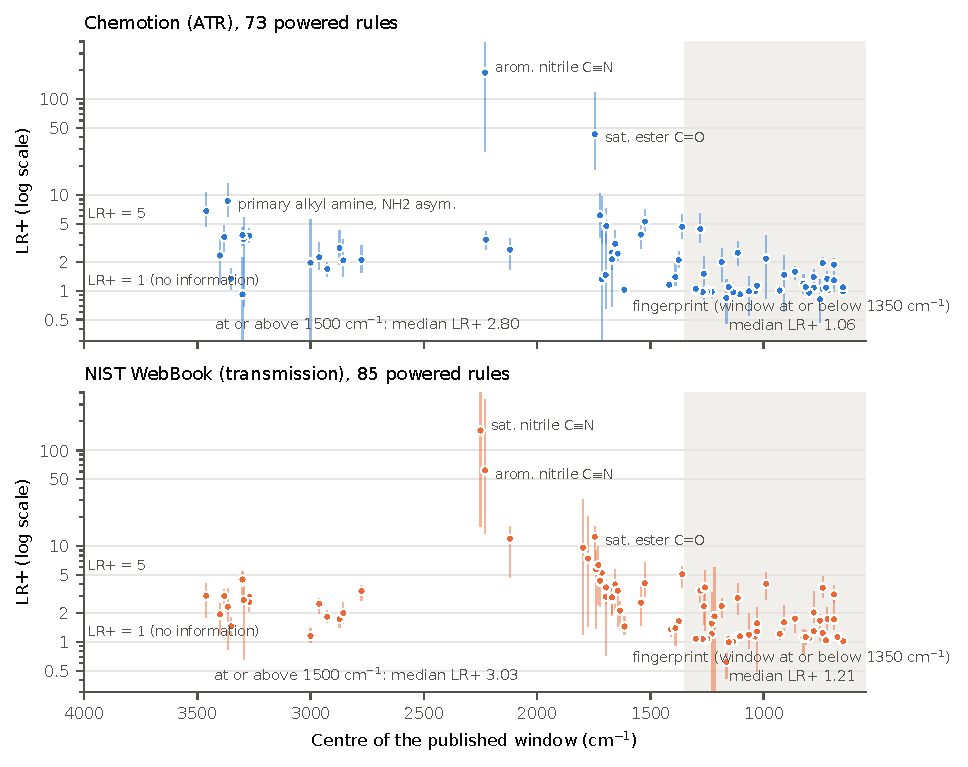
\includegraphics[width=\textwidth]{fig1_lr_by_region}
\caption{Positive likelihood ratio of every powered rule (at least 10 spectra containing the group) against the centre of its published window, in the Chemotion (top) and NIST (bottom) collections. Whiskers are 95\% scaffold-cluster bootstrap intervals; the shaded area marks windows at or below 1350~\wn{}. Median \LRp{} is 2.8 and 3.0 for rules at or above 1500~\wn{}, 1.1 and 1.2 in the fingerprint.}
\label{fig:regions}
\end{figure}

% generated by scripts/tables.py, do not edit by hand
\begin{table}[t]\centering\small
\caption{Number of powered rules in each LR$^+$ band, by spectral region. LR$^+ \geq 5$ is the usual threshold for a test that changes a decision on its own; LR$^+ < 1.2$ means the band is present about as often without the group as with it.}\label{tab:summary}
\begin{tabular}{@{}lrrrrrr@{}}\toprule
Region & $\geq 5$ & 2 to 5 & 1.2 to 2 & $<1.2$ & rules & median LR$^+$ \\
\midrule
\multicolumn{7}{@{}l}{\emph{All powered rules}} \\
\quad Chemotion & 7 & 23 & 14 & 29 & 73 & 1.47 \\
\quad NIST & 10 & 31 & 22 & 22 & 85 & 1.85 \\
\midrule
\multicolumn{7}{@{}l}{\emph{Window at or above 1500 cm$^{-1}$}} \\
\quad Chemotion & 7 & 17 & 5 & 2 & 31 & 2.80 \\
\quad NIST & 9 & 22 & 5 & 1 & 37 & 3.03 \\
\midrule
\multicolumn{7}{@{}l}{\emph{Window straddling 1350--1500 cm$^{-1}$}} \\
\quad Chemotion & 0 & 2 & 1 & 1 & 4 & 1.75 \\
\quad NIST & 1 & 0 & 4 & 0 & 5 & 1.40 \\
\midrule
\multicolumn{7}{@{}l}{\emph{Window at or below 1350 cm$^{-1}$ (fingerprint)}} \\
\quad Chemotion & 0 & 4 & 8 & 26 & 38 & 1.06 \\
\quad NIST & 0 & 9 & 13 & 21 & 43 & 1.21 \\
\bottomrule
\end{tabular}
\end{table}


\subsection{What the intensity clause buys and costs}
\label{sec:intensity}

Forty-nine of the powered rules state an intensity, ``strong'' in all but the nitro scissors (``medium''). Figure~\ref{fig:intensity} compares, for each of them, the \LRp{} obtained from position alone with the \LRp{} obtained when the band must also reach the stated intensity class, defined here as at least 0.6 (strong) or 0.2 (medium) of the strongest band in the spectrum. The clause does what it is meant to do: median specificity rises from 0.39 to 0.85 in Chemotion and from 0.59 to 0.88 in NIST, and \LRp{} improves by more than 20\% in 16 of 20 and 23 of 29 rules. It also does what the tables never mention: median sensitivity falls from 0.78 to 0.44 and from 0.70 to 0.39, and in 8 rules of each collection it is halved or worse.

Whether the trade pays depends on how strong the band really is. Where the group gives one of the strongest bands in the spectrum, the clause costs little and buys a lot: the saturated ester carbonyl goes from 2.9 to 43 while keeping 40 of its 50 percentage points of sensitivity, the aromatic acid carbonyl from 2.4 to 4.8 (0.69 to 0.62), the saturated ketone carbonyl from 3.0 to 5.9 (0.66 to 0.58). Two fingerprint rules are rescued this way: the symmetric nitro stretch at 1330 to 1390~\wn{} and the aromatic ester C-C-O stretch at 1250 to 1310~\wn{} are worthless by position (1.1 in both collections) and become useful with the clause (4.7 and 4.4 in Chemotion, 5.1 and 3.4 in NIST), because a nitro group or an aryl ester does put one of the strongest bands of the spectrum there, and most other compounds do not. Where the band is strong only in the author's memory, the clause removes most true positives: the acid O-H stretch at 2500 to 3500~\wn{} keeps its specificity gain but falls from sensitivity 1.00 to 0.10 (0.44 in NIST), the secondary amide N-H bend from 0.94 to 0.44, the aromatic nitrile from 0.78 to 0.06 (Section~\ref{sec:nitrile}). In four Chemotion rules and one NIST rule the clause lowers \LRp{} outright, which happens when the qualifier removes true positives faster than false ones.

The clause has a second cost that Figure~\ref{fig:intensity} does not show. A rule that misses most true positives loses its value for ruling a group out: in NIST the median \LRn{} of these rules worsens from 0.55 with position alone to 0.72 with the clause, and the number of rules whose \LRn{} exceeds 0.8, that is, whose absence says almost nothing, rises from 4 to 11 of 29. The qualifier turns a rule that worked in both directions into one that works only when the band happens to be strong.

\begin{figure}[t]
\centering
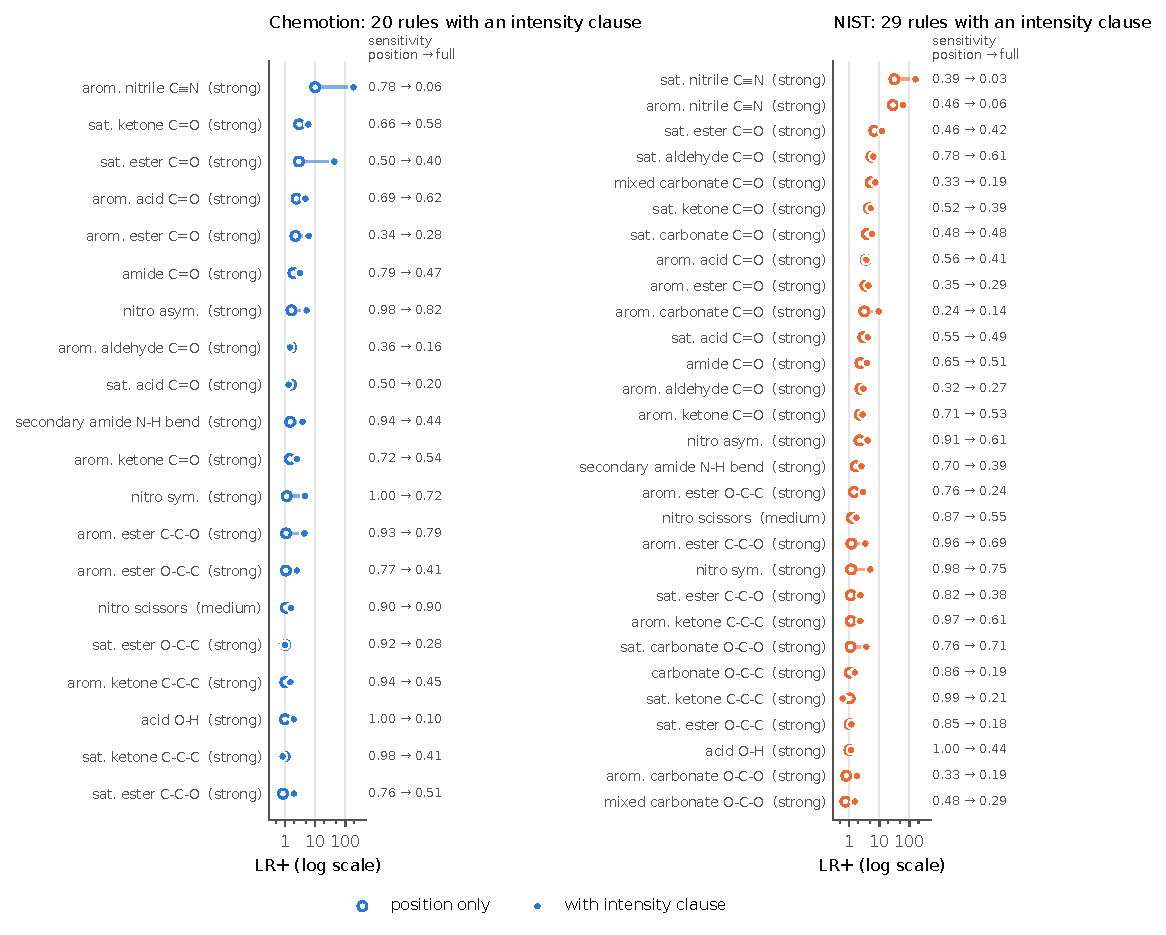
\includegraphics[width=\textwidth]{fig2_position_vs_full}
\caption{Rules that state an intensity: \LRp{} with position alone (open circle) and with the intensity clause applied (filled), in Chemotion (left, 20 rules) and NIST (right, 29 rules). The right-hand column gives the sensitivity before and after the clause. The clause raises \LRp{} in most rules but halves sensitivity or worse in 8 of 20 and 8 of 29.}
\label{fig:intensity}
\end{figure}

\subsection{The nitrile band}
\label{sec:nitrile}

The C$\equiv$N stretch is the clearest case, because the band itself is not in doubt: it is sharp (median width at half height 14~\wn{} in Chemotion, 19 in NIST), it sits in a region of the spectrum where almost nothing else absorbs, and it is detected at the primary threshold in 68 of the 72 Chemotion nitriles and 115 of the 127 NIST nitriles. Yet the published rules, which describe it as ``intense'', recognise 6\% of the aromatic nitriles in Chemotion and 3\% and 6\% of the saturated and aromatic nitriles in NIST.

Figure~\ref{fig:nitrile}a shows why. For each nitrile the height of the C$\equiv$N band relative to the strongest band of its spectrum is a median of 0.30 in Chemotion (interquartile range 0.08 to 0.50) and 0.18 in NIST (0.08 to 0.36); it reaches the ``strong'' class, 0.6 of the strongest band, in one nitrile in ten in either collection (10\% and 11\%). The stretch of a triple bond between two atoms of similar electronegativity carries a modest dipole change, and in a molecule that also has a carbonyl, an ether or an aromatic ring, one of those will provide the strongest band. In Chemotion 19 of the 72 nitriles have the band below 5\% of the maximum; most belong to one family of carbazolyl dicyanobenzenes whose spectra are dominated by the aromatic bands. In NIST 28 of 127 fall below the same level, and they are small, unrelated molecules. Transmission spectra of KBr discs and mulls give the same distribution as ATR spectra of neat solids, so the weakness of the band is a property of the vibration, not of the sampling technique.

Position is a second, smaller problem (Figure~\ref{fig:nitrile}b). The source gives two 20~\wn{} windows, 2220 to 2240 for aromatic and 2240 to 2260 for saturated nitriles. In Chemotion, where the aromatic nitriles come from a few closely related series, 82\% of the apexes fall inside the aromatic window. In NIST they spread from 2190 to 2280~\wn{}, and the windows catch 47\% of the aromatic and 45\% of the saturated nitriles: conjugation, $\alpha$-substitution and the solid state move the band by more than the windows allow. By position alone the rules therefore reach a sensitivity of 0.78 in Chemotion but 0.46 and 0.39 in NIST, with a specificity of 0.92 to 0.99 and an \LRp{} of 10 to 32; the intensity clause then removes what is left.

The numbers that come out of the full rule are a warning about reading \LRp{} alone. With the clause the specificity is 1.00, no non-nitrile ever shows a strong band there, and the \LRp{} is 189 in Chemotion and 62 and 161 in NIST, the highest values in the whole table. A reader who looked only at that column would call the nitrile rule the best in the book. It is, in the sense that a strong band at 2230~\wn{} is proof of a nitrile; it is also a rule that will miss nine nitriles in ten, with an \LRn{} of 0.94 to 0.97 that makes its absence meaningless. What the source means by ``intense'' is, we think, ``conspicuous'': narrow, isolated and impossible to overlook. That is a statement about how easy the band is to notice, not about its height, and the two should not be confused when a rule is written down.

\begin{figure}[t]
\centering
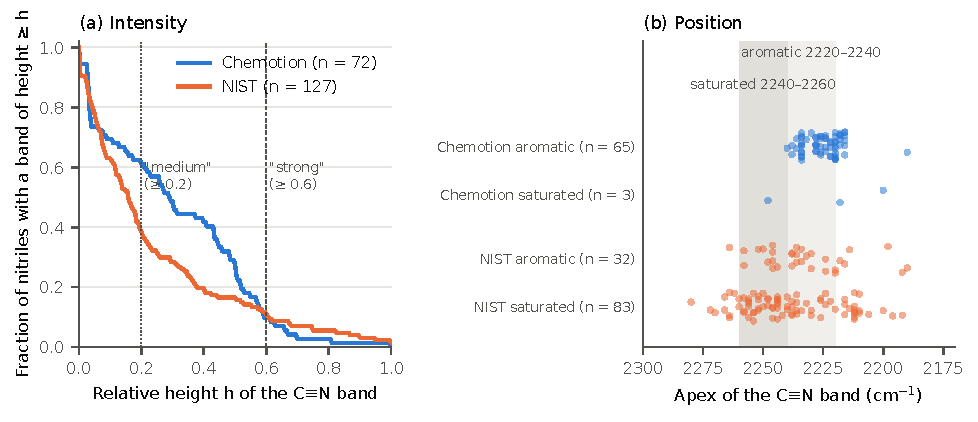
\includegraphics[width=\textwidth]{fig3_nitrile}
\caption{The C$\equiv$N stretch in 72 Chemotion and 127 NIST nitriles. (a) Fraction of nitriles whose band, detected between 2190 and 2280~\wn{}, reaches a given height relative to the strongest band of the spectrum; the dashed lines mark the "medium" and "strong" cut points. One nitrile in ten reaches "strong" in either collection. (b) Apex position by class against the two published windows: the aromatic window catches 82\% of Chemotion but 47\% of NIST aromatic nitriles, the saturated window 45\% of NIST saturated nitriles.}
\label{fig:nitrile}
\end{figure}

\subsection{Benzene substitution patterns}
\label{sec:benzene}

The out-of-plane C-H bending rules for benzene substitution patterns deserve their own figure for two reasons: they are the rules students are taught to trust in the fingerprint, and they are the only rules in the set that combine two bands or use the absence of a band as evidence. Figure~\ref{fig:benzene} gives their \LRp{} and \LRn{} in both collections. Chemotion, with 93\% aromatic compounds and many molecules carrying two or three rings, is the hardest environment these rules could meet; NIST, with 66\% aromatic compounds and mostly one ring per molecule, is closer to the spectra the rules were written from.

As rule-in evidence none of them reaches \LRp{} 5, and most stay below 2. The monosubstituted wag at 710 to 770~\wn{} is found in 97\% of monosubstituted rings and in 93\% of everything else (\LRp{} 1.05 in Chemotion, 1.24 in NIST). The ring bend at 680 to 700~\wn{} does better, 1.9 and 3.1, and asking for both bands adds little (2.0 and 3.7). Every mono and meta rule scores higher in NIST than in Chemotion, and the reason is the denominator: in NIST a third of the compounds have no ring to put a band at 690~\wn{}, whereas in Chemotion 48\% of the compounds that are not monosubstituted still show one.

The two absence rules are the weakest in the table. The ortho rule (wag at 735 to 770, no band at 680 to 700~\wn{}) gives \LRp{} 0.82 in Chemotion, below 1: an ortho-disubstituted compound in this collection is less likely to satisfy the rule than a compound that is not. The reason is that 74\% of the ortho compounds do show a band at 690~\wn{}, against 56\% of the others, because the ortho ring usually carries a monosubstituted phenyl elsewhere in the molecule. In NIST, with simpler molecules, the rule recovers to 1.7 (47\% against 39\%). The para rule behaves the same way (1.2 and 1.1). A rule written for a molecule with one ring turns against itself when the molecule has three.

As rule-out evidence the picture changes. The absence of the 690~\wn{} bend lowers the odds of a monosubstituted ring six-fold (\LRn{} 0.17 and 0.15), and the absence of the meta wag does the same for a meta ring (0.25 and 0.14), because these bands are almost always present when the pattern is (sensitivity 0.89 to 0.98). The ortho and para rules, with \LRn{} 0.7 to 1.1, are uninformative in both directions. The substitution rules, then, do not identify a pattern; when the expected band is missing, they exclude one, and that is the use a spectroscopist can still make of them.

\begin{figure}[t]
\centering
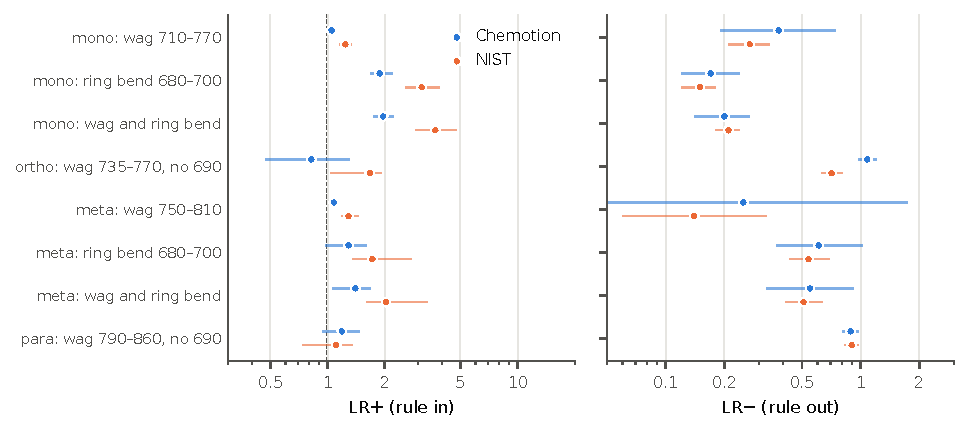
\includegraphics[width=\textwidth]{fig4_benzene}
\caption{Rule-in (\LRp{}) and rule-out (\LRn{}) value of the out-of-plane bending rules for benzene substitution patterns, with 95\% intervals, in both collections. No pattern reaches \LRp{} 5; the ring bend at 690~\wn{} and its combination with the wag are the only rules above 2, and only in NIST. The monosubstituted ring bend is a useful rule-out (\LRn{} 0.17 and 0.15).}
\label{fig:benzene}
\end{figure}

\subsection{Rule-out value}
\label{sec:ruleout}

The tables read in one direction, from band to group; the likelihood ratios read in both. Of the 73 and 85 powered rules, 11 and 17 have an \LRn{} of 0.3 or lower, that is, their absence lowers the odds of the group at least three-fold, and 25 and 24 have an \LRn{} of 0.8 or higher, so that their absence means almost nothing. Only one rule, the terminal alkyne C-H stretch at 3250 to 3350~\wn{}, is useful in both directions in both collections (\LRp{} 3.8 and 4.5, \LRn{} 0.17 and 0.06): the band is present in 87\% and 96\% of terminal alkynes and in about a fifth of everything else. The other reliable rule-outs are the secondary amide N-H stretch (\LRn{} 0.08 in Chemotion; 0.33 in NIST, where hydrogen-bonded solids broaden it), the primary amide N-H stretches (0.10 in NIST), the primary amine NH$_2$ scissors (0.11), the monosubstituted benzene ring bend (0.17 and 0.15) and the meta wag (0.25 and 0.14).

An \LRn{} is only usable when the negative result actually occurs. Several fingerprint rules have an \LRn{} below 0.2 with an \LRp{} of about 1, for instance the tertiary alcohol C-O stretch at 1100 to 1210~\wn{} in NIST (\LRn{} 0.08, \LRp{} 1.07), and this is not a contradiction: the band is present in every tertiary alcohol and in 93\% of the other compounds, so its absence does rule the group out, but the absence is seen in one spectrum in fourteen. These rules are listed in Table~\ref{tab:rules} with their specificity, which is the number that tells the reader how often the rule-out can be invoked.

\subsection{Agreement between collections}
\label{sec:replication}

Everything above could be a property of one laboratory, one instrument and one sampling technique. Figure~\ref{fig:replication} plots, for the 71 rules powered in both collections, the \LRp{} in Chemotion against the \LRp{} in NIST. The rank correlation is 0.79, and 62 of the 71 rules (87\%) agree within a factor of two, with the fingerprint rules clustered around (1, 1) and the carbonyl, N-H and C$\equiv$X rules rising along the diagonal. Two collections that share no compound, no instrument, no sampling technique and no decade order the rules the same way.

The nine rules that disagree by more than a factor of two are labelled, and each has a reading. Six involve groups that are rare or narrowly represented in Chemotion: the saturated primary and secondary amines (13 and 24 positives), the saturated acid (10) and the aromatic aldehyde (64, with a wide interval), where the Chemotion estimate is simply uncertain, and the two primary amine NH$_2$ stretches (13 and 61 positives), which score higher in Chemotion than in NIST in the direction expected from hydrogen bonding: in KBr discs and mulls the N-H bands of amines broaden and shift down, out of the narrow windows. Two are chemistry of the collection rather than of the rule: the saturated ester carbonyl falls from 43 to 12 because NIST holds many more anhydrides, lactones and acids that place a strong band in the same window, and the terminal alkyne C$\equiv$C rises from 2.7 to 12 because the Chemotion alkynes are mostly conjugated aryl alkynes whose band sits above the 2100 to 2140~\wn{} window. The ninth is the ortho absence rule of Section~\ref{sec:benzene}. No rule changes sign: what is evidence in one collection is evidence in the other, and what is noise is noise.

Agreement is weaker for \LRn{} (72\% within a factor of two), because \LRn{} depends on sensitivity, and sensitivity depends on which members of a group a collection happens to contain: the secondary amide N-H stretch is found in 94\% of Chemotion amides but 75\% of NIST amides, most of which are hydrogen-bonded solids. Rule-in value travels between collections better than rule-out value, and the rule-out figures in Table~\ref{tab:rules} should be read with that in mind.

\begin{figure}[t]
\centering
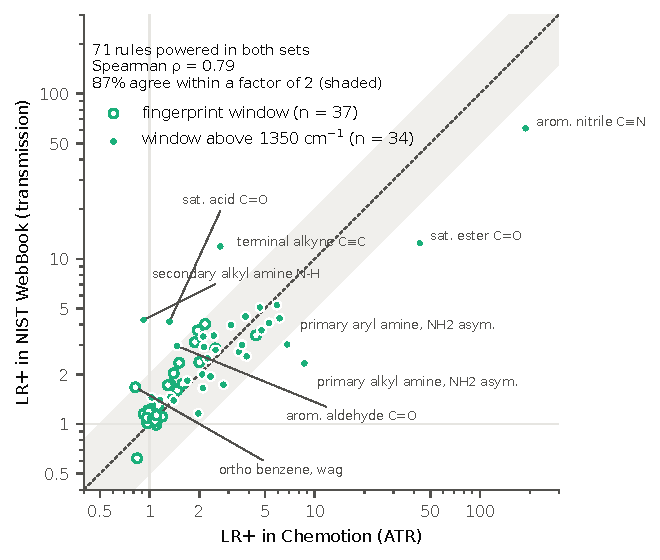
\includegraphics[width=0.7\textwidth]{fig5_replication}
\caption{\LRp{} of the 71 rules powered in both collections, Chemotion against NIST. The shaded band is agreement within a factor of two (62 of 71 rules, 87\%); Spearman correlation 0.79. Labelled rules disagree by more than a factor of two; six of the nine involve a group with fewer than 30 positives in Chemotion.}
\label{fig:replication}
\end{figure}

\section{Discussion}
\label{sec:discussion}

The standard texts on infrared interpretation describe the region below about 1400~\wn{} as complex and rarely diagnostic on its own, and the carbonyl and X-H regions as the place where group frequencies are reliable~\cite{colthup1990introduction,bellamy1975infrared}. That description is correct, and this study gives it numbers: above 1500~\wn{} the median rule multiplies the odds of its group by three, and the best ones by ten or forty; below 1350~\wn{} the median rule multiplies them by one. What the description does not give, because the counting had not been done at this scale, is how uniform the failure is (26 of 38 fingerprint rules below 1.2 in Chemotion), that the exceptions are exactly the rules that ask for more than a position, and that a rule which is useless for confirming a group can still be good for excluding it. The absence of the 690~\wn{} ring bend, of the secondary amide N-H stretch or of the terminal alkyne C-H stretch each lower the odds of their group by a factor of six to seventeen, a direction the tables do not list. The expert systems that once encoded these tables did attach a confidence to each rule~\cite{woodruff1980pairs,andreev1996expirs}, but it was the author's estimate; the values reported here are measured, and they can be re-measured on any other collection.

The tables could not have said it, and the reason is structural. A correlation table is built from spectra of compounds that have the group: it records where the band is and roughly how it looks. It has no denominator. Sensitivity can be estimated from such a collection, specificity cannot, and it is specificity that the fingerprint lacks. A second reason is that the rules were written for a reader looking at a whole spectrum, who weighs each band against its neighbours, notices patterns and discards what does not fit; nobody applies the C-O rule for secondary alcohols in isolation. We tested each rule on its own, which is what a student does with a table on the first day and what any program does that encodes the table literally. The likelihood ratios reported here are therefore a fair measure of the rules as written, a lower bound for what an experienced reader extracts from the same bands, and a warning to anyone who would automate the table one row at a time.

Table~\ref{tab:failures} groups the rules that carry no evidence in either collection by what fills their window. Eleven are single-bond C-O and C-N stretches between 1000 and 1350~\wn{}; their false positives are dominated by aryl esters, aryl ethers and aromatic ketones, whose C-O and aryl-C(=O) stretches sit in the same windows with odds ratios of 10 to 44. Six are bending and wagging modes between 600 and 860~\wn{}, filled by the C-H wags of monosubstituted and para rings. Two are fingerprint rules whose ``strong'' qualifier removes true positives faster than false ones. Beyond these, three failure modes recur in rules that do carry evidence: intensity qualifiers on bands that are not in fact strong (Section~\ref{sec:intensity}), windows narrower than the spread of the band across the group (the nitrile windows catch half of the NIST nitriles; the terminal alkyne C$\equiv$C window misses the conjugated alkynes of Chemotion), and absence conditions that a second ring in the molecule violates.

\begin{table}[t]
\centering\small
\caption{Failure modes of the frozen rules. The first three rows cover the 19 group rules with \LRp{} below 1.2 in both collections; the last three recur in rules that carry evidence. Odds ratios are those of the groups most over-represented among the false positives (NIST, primary threshold).}
\label{tab:failures}
\begin{tabular}{@{}p{3.6cm}p{4.6cm}p{6.6cm}@{}}
\toprule
Failure mode & Rules affected & What the data show \\
\midrule
Single-bond C-O and C-N stretches, 1000 to 1350~\wn{} & 11 rules: C-O of primary, secondary and tertiary alcohols, phenols, saturated, aryl alkyl and diaryl ethers, acids; C-N of primary and secondary amines and secondary amides & Sensitivity 0.9 to 1.0, specificity 0.01 to 0.16. Almost every spectrum has a band in the window; false positives are dominated by aryl esters (OR 11 to 44), aryl ethers (8 to 15) and aromatic ketones (8 to 44), whose own C-O and aryl-C(=O) stretches fall there. \\
Bending and wagging modes, 600 to 860~\wn{} & 6 rules: alcohol O-H wag, primary and secondary amine N-H wags, secondary amide N-H wag, para-disubstituted benzene wag, trisubstituted alkene wag & Filled by the aromatic C-H wags: monosubstituted rings (OR 11 to 43) and para rings (OR 5 to 64) among the false positives. In Chemotion, with 93\% aromatic compounds, specificity 0.02 to 0.16. \\
``Strong'' qualifier that reverses the sign & 2 rules: saturated ketone C-C-C (1100 to 1230), saturated ester O-C-C (1030 to 1100) & The band is present in 85 to 99\% of the group by position but reaches the strong class in 18 to 42\%; the qualifier removes true positives faster than false ones and \LRp{} falls to 0.6 to 1.2. \\
\midrule
Intensity qualifier on a band that is not strong & Nitrile C$\equiv$N (both classes), acid O-H stretch, secondary amide N-H bend, ester and ketone skeletal stretches & Specificity rises to 0.85 to 1.00 but sensitivity falls to 0.03 to 0.44; \LRp{} looks excellent while the rule misses most of the group and \LRn{} approaches 1 (Sections~\ref{sec:intensity} and \ref{sec:nitrile}). \\
Window narrower than the spread of the band & Nitrile windows (20~\wn{}); terminal alkyne C$\equiv$C 2100 to 2140 & By position alone the nitrile windows catch 45 to 47\% of NIST nitriles; the Chemotion alkynes, mostly conjugated, sit above the C$\equiv$C window (\LRp{} 2.7 against 12 in NIST). \\
Absence condition violated by a second ring & Ortho and para benzene rules (no band at 680 to 700~\wn{}) & 74\% of Chemotion ortho compounds show the forbidden band, against 56\% of the others, because the molecule carries a monosubstituted phenyl elsewhere; \LRp{} 0.82. \\
\bottomrule
\end{tabular}
\end{table}

On the intensity words we make one concrete suggestion. ``Strong'', ``medium'' and ``weak'' in the tables describe how a band looks to the eye in a transmission spectrum of a small molecule, and as such they are useful. They are not thresholds, and the nitrile shows what happens when they are read as thresholds. A rule that is meant to be applied literally, by a student or a program, should state what it means: either a relative height (the ester carbonyl, when it falls in its window, is above 0.6 of the strongest band in 80 to 90\% of esters; the nitrile stretch is above 0.2 in 43 to 65\% of nitriles and above 0.6 in one in ten) or a word that describes the right property, and for the nitrile that word is ``sharp'' or ``isolated'', not ``intense''. Table~\ref{tab:rules} and the released result tables give the relative heights that would let the qualifiers be rewritten this way for every rule in the set.

The table is meant to be used the way likelihood ratios are used in diagnosis. A reader who suspects an ester from the reaction and sees a strong band at 1740~\wn{} multiplies the odds by 43 (12 in a collection rich in other carbonyls) and can stop; a reader who sees a band at 1100~\wn{} has learned almost nothing and should look elsewhere; a reader who does not see a band at 690~\wn{} can set the monosubstituted ring aside. Two cautions come with this. \LRp{} depends on what else is in the collection, and the two collections show how far it moves: within a factor of two for most rules, but from 43 to 12 for the ester when anhydrides and lactones enter the picture. And \LRn{} depends on which members of a group the collection holds, and travels less well than \LRp{}; the rule-out values should be taken as indicative until they are replicated on further collections.

The study has limits that the reader should weigh. The rules come from one source; other tables give other windows, and the audit says nothing about them, although the method applies to any of them unchanged. Ground truth is the deposited structure matched by our SMARTS definitions, which encode one reading of the source's group names; a different reading of ``saturated'' or ``aromatic'' would move some rules. Band detection is a fixed algorithm with a fixed threshold, and the height measure it uses penalises bands that are strong in area but low in height, the acid O-H envelope above all. Chemotion is an ATR collection with a 93\% aromatic, synthesis-laboratory composition; NIST pools KBr, mull, solution and neat spectra from several decades of instruments, and 43\% of its primary spectra are digitised micrometre scans; we did not stratify by preparation, and mulls in particular add hydrocarbon bands that inflate the methyl and methylene false positives. Each rule was scored alone, without the context a human reader uses. No correction for multiple comparisons was made, and none is claimed. What survives these limits is the pattern: two collections that share none of them agree on it.

Three extensions follow. Other rule sources, and in particular the tables of the classic monographs, can be transcribed and scored with the same scripts against the same collections, which would show how much the sources agree once they are measured rather than compared by eye. Combinations of rules, which is how the fingerprint is actually read, can be scored the same way, with the frozen set as the starting point. And any laboratory with a collection of spectra and structures can compute its own column of the table, which is the only way the composition dependence of the ratios can be mapped. The rule table, the definitions and the scripts are released so that this can be done without re-deriving them.

\section{Conclusions}
\label{sec:conclusions}

Scored as diagnostic tests on 6,663 experimental spectra with known structures, the classical infrared correlation rules divide into two regimes. At or above 1500~\wn{} most rules carry real evidence, with a median positive likelihood ratio of about 3 and values up to 43 for the saturated ester carbonyl; at or below 1350~\wn{} band position alone is close to uninformative, with a median ratio of 1.1 to 1.2, because almost every spectrum has a band in almost every window. Two collections that share no compound, instrument, sampling technique or decade rank the rules the same way (Spearman 0.79; 87\% within a factor of two). Intensity qualifiers raise specificity but cost more sensitivity than the tables acknowledge, and for the nitrile stretch the word ``intense'' turns the most conspicuous band in the spectrum into a rule that recognises one nitrile in ten. Several rules, including the benzene substitution patterns, are of little use for confirming a group but good for excluding it, a direction the tables do not list. The quantified table, the frozen rule set and the scripts are released so that the audit can be extended to other sources and other collections.

\section*{Data and code availability}
The Chemotion IR collection is available under CC BY-SA 4.0 at RADAR4Chem (DOI 10.22000/OGoEQGlsZGElrgst). NIST Chemistry WebBook spectra (SRD 69) are subject to NIST's terms of use and are not redistributed; the download script and the list of identifiers used are provided. The frozen rule set, the SMARTS definitions, the processing and evaluation scripts, and the per-rule result tables are available at \todo{repository URL}, tag \texttt{rules-frozen-v1}.

\section*{Competing interests}
The author is the founder of Mol Insight S.L., which develops software for spectral interpretation. The rule set, the analysis and the conclusions of this work do not depend on that software, and the study did not use it.

\section*{Author contributions}
K.I.C. conceived the study, built the pipeline, performed the analysis and wrote the manuscript.

\section*{Acknowledgements}
The author thanks the Chemotion team for releasing the IR collection with structures under an open licence, and Brian C. Smith, whose column made a consistent, fully documented rule set available to transcribe.

\section*{Declaration of generative AI use}
A large language model (Claude, Anthropic) was used to draft English text from the author's notes and outline, and to write analysis code under the author's direction. The author reviewed, verified and edited all text and code and takes full responsibility for the content of the manuscript.


\bibliographystyle{unsrtnat}
\bibliography{refs}

\clearpage
\appendix
\setcounter{table}{0}
\renewcommand{\thetable}{A\arabic{table}}
\section{Quantified rule table}
\label{app:table}
\small
% generated by scripts/tables.py, do not edit by hand
\begingroup\footnotesize\setlength{\tabcolsep}{4pt}
\begin{longtable}{@{}>{\raggedright\arraybackslash}p{2.5cm}>{\raggedright\arraybackslash}p{6.6cm}rrrrrrrr@{}}
\caption{Diagnostic value of the frozen correlation rules (group tier) in the two collections. Window, stated intensity and description as transcribed from the source; $n_+$, number of spectra containing the group; LR$^+$ and LR$^-$ at the primary threshold with the full rule definition. Values in parentheses are underpowered (fewer than 10 positives) and are shown for completeness only.}\label{tab:rules}\\
\toprule
 & & & \multicolumn{3}{c}{Chemotion (ATR)} & & \multicolumn{3}{c}{NIST WebBook} \\
\cmidrule(lr){4-6}\cmidrule(lr){8-10}
Group & Band (cm$^{-1}$, intensity) & & $n_+$ & LR$^+$ & LR$^-$ & & $n_+$ & LR$^+$ & LR$^-$ \\
\midrule
\endfirsthead
\toprule
 & & & \multicolumn{3}{c}{Chemotion (ATR)} & & \multicolumn{3}{c}{NIST WebBook} \\
\cmidrule(lr){4-6}\cmidrule(lr){8-10}
Group & Band (cm$^{-1}$, intensity) & & $n_+$ & LR$^+$ & LR$^-$ & & $n_+$ & LR$^+$ & LR$^-$ \\
\midrule
\endhead
\midrule\multicolumn{10}{r}{\small continued on the next page}\\
\endfoot
\bottomrule
\endlastfoot
primary aryl amine & 3420--3500; {\scriptsize NH2 asymmetric stretch of an aromatic primary amine} & & 61 & 6.8 & 0.40 & & 361 & 3.0 & 0.61 \\
secondary aryl amine & 3380--3420; {\scriptsize N-H stretch of an aromatic secondary amine, one band} & & 60 & 2.3 & 0.82 & & 191 & 1.9 & 0.87 \\
primary alkyl amine & 3350--3380; {\scriptsize NH2 asymmetric stretch of a saturated primary amine} & & 13 & 8.7 & 0.33 & & 111 & 2.3 & 0.87 \\
primary aryl amine & 3340--3420; {\scriptsize NH2 symmetric stretch of an aromatic primary amine} & & 61 & 3.6 & 0.35 & & 361 & 3.0 & 0.46 \\
alcohol & 3300--3400, broad; {\scriptsize O-H stretch of alcohols and phenols} & & 181 & 1.3 & 0.88 & & 1194 & 1.5 & 0.86 \\
secondary alkyl amine & 3280--3320; {\scriptsize N-H stretch of a saturated secondary amine, one band} & & 24 & 0.9 & 1.01 & & 74 & 4.3 & 0.66 \\
primary alkyl amine & 3280--3310; {\scriptsize NH2 symmetric stretch of a saturated primary amine} & & 13 & 3.5 & 0.69 & & 111 & 2.7 & 0.86 \\
terminal alkyne & 3250--3350; {\scriptsize Alkyne C-H stretch of a monosubstituted (terminal) alkyne} & & 23 & 3.8 & 0.17 & & 23 & 4.5 & 0.06 \\
primary amide & 3170--3370; {\scriptsize N-H stretches of a primary amide, two bands} & & 5 & (1.3) & (0.88) & & 100 & 2.9 & 0.10 \\
secondary amide & 3170--3370; {\scriptsize N-H stretch of a secondary amide, one band} & & 147 & 3.8 & 0.08 & & 356 & 2.6 & 0.33 \\
methyl & 2952--2972; {\scriptsize Asymmetric C-H stretch of the methyl group} & & 1069 & 2.2 & 0.68 & & 3136 & 2.5 & 0.78 \\
methylene & 2916--2936; {\scriptsize Asymmetric C-H stretch of the methylene group} & & 1007 & 1.7 & 0.52 & & 3017 & 1.8 & 0.83 \\
methyl & 2862--2882; {\scriptsize Symmetric C-H stretch of the methyl group} & & 1069 & 2.8 & 0.79 & & 3136 & 1.7 & 0.89 \\
methylene & 2845--2865; {\scriptsize Symmetric C-H stretch of the methylene group} & & 1007 & 2.1 & 0.73 & & 3017 & 2.0 & 0.89 \\
aldehyde & 2700--2850; {\scriptsize Aldehydic C-H stretch, typically a doublet} & & 68 & 2.1 & 0.56 & & 72 & 3.4 & 0.38 \\
carboxylic acid & 2500--3500, strong, broad; {\scriptsize O-H stretch envelope of a carboxylic acid dimer} & & 48 & 2.0 & 0.95 & & 325 & 1.2 & 0.90 \\
saturated nitrile & 2240--2260, strong, sharp; {\scriptsize C-N triple bond stretch of a saturated nitrile} & & 3 & (384) & (0.88) & & 94 & 161 & 0.97 \\
aromatic nitrile & 2220--2240, strong, sharp; {\scriptsize C-N triple bond stretch of an aromatic nitrile} & & 69 & 189 & 0.94 & & 33 & 62 & 0.94 \\
internal alkyne & 2190--2260; {\scriptsize C-C triple bond stretch of a disubstituted alkyne} & & 79 & 3.4 & 0.28 & & 9 & (5.9) & (0.71) \\
terminal alkyne & 2100--2140; {\scriptsize C-C triple bond stretch of a monosubstituted alkyne} & & 23 & 2.7 & 0.41 & & 23 & 12 & 0.67 \\
organic carbonate & 1775--1820, strong; {\scriptsize C$=$O stretch of an aromatic organic carbonate} & & 2 & (30) & (0.84) & & 21 & 9.6 & 0.87 \\
organic carbonate & 1760--1790, strong; {\scriptsize C$=$O stretch of a mixed organic carbonate} & & 2 & (34) & (0.84) & & 21 & 7.4 & 0.83 \\
saturated ester & 1735--1755, strong; {\scriptsize C$=$O stretch of a saturated ester} & & 128 & 43 & 0.61 & & 440 & 12 & 0.60 \\
organic carbonate & 1730--1750, strong; {\scriptsize C$=$O stretch of a saturated organic carbonate} & & 2 & (2.6) & (0.89) & & 21 & 5.7 & 0.57 \\
saturated aldehyde & 1720--1740, strong; {\scriptsize C$=$O stretch of a saturated aldehyde} & & 3 & (1.7) & (0.94) & & 18 & 6.3 & 0.43 \\
aromatic ester & 1715--1730, strong; {\scriptsize C$=$O stretch of an aromatic ester} & & 116 & 6.1 & 0.75 & & 169 & 4.4 & 0.76 \\
saturated ketone & 1705--1725, strong; {\scriptsize C$=$O stretch of a saturated ketone} & & 41 & 5.9 & 0.46 & & 173 & 5.2 & 0.66 \\
saturated carboxylic acid & 1700--1730, strong; {\scriptsize C$=$O stretch of a saturated carboxylic acid} & & 10 & 1.3 & 0.94 & & 211 & 4.2 & 0.58 \\
aromatic aldehyde & 1685--1710, strong; {\scriptsize C$=$O stretch of an aromatic aldehyde} & & 64 & 1.5 & 0.94 & & 44 & 3.0 & 0.80 \\
aromatic carboxylic acid & 1680--1710, strong; {\scriptsize C$=$O stretch of an aromatic carboxylic acid} & & 29 & 4.8 & 0.44 & & 91 & 3.7 & 0.67 \\
trisubstituted alkene & 1660--1680; {\scriptsize C$=$C stretch of a trisubstituted alkene} & & 41 & 2.1 & 0.73 & & 158 & 2.9 & 0.73 \\
aromatic ketone & 1640--1700, strong; {\scriptsize C$=$O stretch of an aromatic ketone} & & 159 & 2.5 & 0.59 & & 219 & 2.8 & 0.58 \\
amide & 1630--1680, strong; {\scriptsize C$=$O stretch of any amide (amide I)} & & 223 & 3.1 & 0.62 & & 635 & 4.0 & 0.57 \\
vinyl alkene & 1630--1660; {\scriptsize C$=$C stretch of a vinyl group} & & 34 & 2.5 & 0.34 & & 91 & 3.4 & 0.34 \\
primary amide & 1620--1650; {\scriptsize NH2 scissors of a primary amide} & & 5 & (0.7) & (1.14) & & 100 & 2.1 & 0.62 \\
primary amine & 1580--1650, broad; {\scriptsize NH2 scissors of a primary amine} & & 76 & 1.0 & 0.81 & & 490 & 1.4 & 0.11 \\
secondary amide & 1515--1570, strong; {\scriptsize N-H in-plane bend of a secondary amide (amide II)} & & 147 & 3.9 & 0.63 & & 356 & 2.6 & 0.72 \\
nitro & 1500--1550, strong; {\scriptsize Asymmetric NO2 stretch} & & 50 & 5.3 & 0.21 & & 388 & 4.1 & 0.46 \\
carboxylic acid & 1395--1440; {\scriptsize O-H in-plane bend of a carboxylic acid} & & 48 & 1.2 & 0.33 & & 325 & 1.4 & 0.36 \\
primary amide & 1390--1430; {\scriptsize C-N stretch of a primary amide} & & 5 & (0.8) & (1.62) & & 100 & 1.4 & 0.52 \\
aldehyde & 1380--1400; {\scriptsize Aldehydic C-H bend} & & 68 & 1.4 & 0.71 & & 72 & 1.4 & 0.71 \\
methyl & 1365--1385; {\scriptsize Symmetric bend (umbrella mode) of the methyl group} & & 1069 & 2.1 & 0.55 & & 3136 & 1.6 & 0.60 \\
nitro & 1330--1390, strong; {\scriptsize Symmetric NO2 stretch} & & 50 & 4.7 & 0.33 & & 388 & 5.1 & 0.29 \\
secondary aryl amine & 1250--1350; {\scriptsize C-N-C asymmetric stretch of an aromatic secondary amine} & & 60 & 1.1 & 0.28 & & 191 & 1.1 & 0.17 \\
primary aryl amine & 1250--1350; {\scriptsize C-N stretch of an aromatic primary amine} & & 61 & 1.0 & 0.84 & & 361 & 1.1 & 0.24 \\
aromatic ester & 1250--1310, strong; {\scriptsize C-C-O stretch of an aromatic ester} & & 116 & 4.4 & 0.25 & & 169 & 3.4 & 0.39 \\
organic carbonate & 1240--1280, strong; {\scriptsize O-C-O asymmetric stretch of a saturated organic carbonate} & & 2 & (2.2) & (0.64) & & 21 & 3.7 & 0.35 \\
secondary amide & 1230--1310; {\scriptsize C-N stretch of a secondary amide} & & 147 & 1.0 & 1.49 & & 356 & 1.1 & 0.45 \\
aromatic ketone & 1230--1300, strong; {\scriptsize C-C-C asymmetric stretch of an aromatic ketone} & & 159 & 1.5 & 0.79 & & 219 & 2.4 & 0.53 \\
carboxylic acid & 1210--1320; {\scriptsize C-O stretch of a carboxylic acid} & & 48 & 1.0 & 3.33 & & 325 & 1.0 & 0.42 \\
organic carbonate & 1210--1250, strong; {\scriptsize O-C-O stretch of a mixed organic carbonate} & & 2 & (3.1) & (0.23) & & 21 & 1.6 & 0.87 \\
organic carbonate & 1205--1230, strong; {\scriptsize O-C-O stretch of an aromatic organic carbonate} & & 2 & (4.8) & (0.20) & & 21 & 1.9 & 0.90 \\
phenol & 1200--1260; {\scriptsize C-O stretch of a phenol} & & 64 & 1.0 & 1.21 & & 422 & 1.2 & 0.23 \\
aryl alkyl ether & 1200--1300; {\scriptsize Aromatic C-O stretch of a mixed (alkyl aryl) ether} & & 229 & 1.0 & 0.57 & & 346 & 1.1 & 0.22 \\
diaryl ether & 1200--1300; {\scriptsize C-O stretch of a diaryl ether, one band} & & 13 & 1.0 & 2.42 & & 89 & 1.1 & 0.07 \\
saturated ester & 1160--1210, strong; {\scriptsize C-C-O stretch of a saturated ester} & & 128 & 2.0 & 0.66 & & 440 & 2.4 & 0.74 \\
secondary alkyl amine & 1130--1180; {\scriptsize C-N-C asymmetric stretch of a saturated secondary amine} & & 24 & 1.1 & 0.18 & & 74 & 1.0 & 1.03 \\
aromatic ester & 1100--1130, strong; {\scriptsize O-C-C stretch of an aromatic ester} & & 116 & 2.5 & 0.70 & & 169 & 2.9 & 0.83 \\
saturated ketone & 1100--1230, strong; {\scriptsize C-C-C asymmetric stretch of a saturated ketone} & & 41 & 0.8 & 1.16 & & 173 & 0.6 & 1.19 \\
tertiary alcohol & 1100--1210; {\scriptsize C-O stretch of a tertiary alcohol} & & 8 & (1.0) & (3.62) & & 94 & 1.1 & 0.08 \\
secondary alcohol & 1075--1150; {\scriptsize C-O stretch of a secondary alcohol} & & 47 & 1.0 & 1.42 & & 259 & 1.1 & 0.23 \\
saturated ether & 1070--1140; {\scriptsize C-O stretch of a saturated ether, one band} & & 83 & 0.9 & 2.54 & & 242 & 1.1 & 0.19 \\
saturated ester & 1030--1100, strong; {\scriptsize O-C-C asymmetric stretch of a saturated ester} & & 128 & 1.0 & 1.01 & & 440 & 1.2 & 0.97 \\
primary alkyl amine & 1020--1250; {\scriptsize C-N stretch of a saturated primary amine} & & 13 & 1.0 & 15.58 & & 111 & 1.0 & 0.43 \\
aryl alkyl ether & 1010--1050; {\scriptsize Saturated C-O stretch of a mixed (alkyl aryl) ether} & & 229 & 1.1 & 0.36 & & 346 & 1.3 & 0.35 \\
primary alcohol & 1000--1075; {\scriptsize C-O stretch of a primary alcohol} & & 20 & 1.0 & 1.23 & & 232 & 1.1 & 0.18 \\
organic carbonate & 1000--1060, strong; {\scriptsize O-C-C stretch of any organic carbonate} & & 2 & (2.1) & (0.65) & & 21 & 1.6 & 0.92 \\
vinyl alkene & 985--995; {\scriptsize First C-H wag of a vinyl group} & & 34 & 2.2 & 0.77 & & 91 & 4.0 & 0.54 \\
vinyl alkene & 905--915; {\scriptsize Second C-H wag of a vinyl group} & & 34 & 1.5 & 0.84 & & 91 & 1.6 & 0.88 \\
carboxylic acid & 900--960, broad; {\scriptsize O-H out-of-plane bend (wag) of a carboxylic acid} & & 48 & 1.0 & 0.93 & & 325 & 1.2 & 0.44 \\
nitro & 835--890, medium; {\scriptsize NO2 scissors bend} & & 50 & 1.6 & 0.23 & & 388 & 1.8 & 0.66 \\
trisubstituted alkene & 790--840; {\scriptsize C-H wag of a trisubstituted alkene} & & 41 & 1.1 & 0.46 & & 158 & 1.1 & 0.75 \\
benzene, para & 790--860, no band 680--700; {\scriptsize Out-of-plane C-H bending of a para-disubstituted benzene ring} & & 415 & 1.2 & 0.89 & & 645 & 1.1 & 0.90 \\
benzene, meta & 750--810 + band 680--700; {\scriptsize Out-of-plane C-H bending of a meta-disubstituted benzene ring together with the ring bend at 690+-10 (the rule as printed in Table III)} & & 42 & 1.4 & 0.55 & & 141 & 2.0 & 0.51 \\
primary amine & 750--850, broad; {\scriptsize NH2 out-of-plane bend (wag) of a primary amine} & & 76 & 1.0 & 2.96 & & 490 & 1.1 & 0.35 \\
benzene, meta & 750--810; {\scriptsize Out-of-plane C-H bending of a meta-disubstituted benzene ring} & & 42 & 1.1 & 0.25 & & 141 & 1.3 & 0.14 \\
benzene, ortho & 735--770, no band 680--700; {\scriptsize Out-of-plane C-H bending of an ortho-disubstituted benzene ring} & & 145 & 0.8 & 1.08 & & 258 & 1.7 & 0.71 \\
(CH$\_2$)$\_{n\geq4}$ chain & 710--730; {\scriptsize Rocking vibration of the methylene group} & & 130 & 1.3 & 0.58 & & 632 & 1.7 & 0.62 \\
benzene, monosubstituted & 710--770; {\scriptsize Out-of-plane C-H bending of a monosubstituted benzene ring} & & 344 & 1.1 & 0.38 & & 928 & 1.2 & 0.27 \\
benzene, monosubstituted & 710--770 + band 680--700; {\scriptsize Out-of-plane C-H bending of a monosubstituted benzene ring together with the ring bend at 690+-10 (the rule as printed in Table III)} & & 344 & 2.0 & 0.20 & & 924 & 3.7 & 0.21 \\
secondary amine & 700--750; {\scriptsize N-H wag of a secondary amine} & & 85 & 1.1 & 0.33 & & 281 & 1.0 & 0.91 \\
benzene, monosubstituted & 680--700; {\scriptsize Ring bend at 690 present for a monosubstituted benzene ring} & & 344 & 1.9 & 0.17 & & 924 & 3.1 & 0.15 \\
benzene, meta & 680--700; {\scriptsize Ring bend at 690 present for a meta-disubstituted benzene ring} & & 42 & 1.3 & 0.61 & & 141 & 1.7 & 0.54 \\
secondary amide & 680--750, broad; {\scriptsize N-H out-of-plane bend of a secondary amide} & & 147 & 1.0 & 0.57 & & 354 & 1.1 & 0.70 \\
alcohol & 600--700, broad; {\scriptsize O-H wag (out-of-plane bend) of alcohols and phenols} & & 181 & 1.0 & 1.06 & & 391 & 1.0 & 0.97 \\
primary amide & 600--750, broad; {\scriptsize NH2 wag of a primary amide} & & 5 & (0.9) & (3.82) & & 39 & 1.1 & 0.32 \\
terminal alkyne & 600--700; {\scriptsize Alkyne C-H bend of a monosubstituted alkyne} & & 23 & 1.1 & 0.55 & & 1 & (1.3) & (0.59) \\
\end{longtable}\endgroup


\end{document}
